\section{正则化}
\label{sec:chapter5}

\subsection{过拟合}

以多项式回归为例。多项式回归是指在线性回归的基础上，人为的引入高阶项并将其视为新的一维特征，然后进行线性回归，从而达到拟合非线性数据的目的。举例而言，设线性回归的一个数据是 $\left(x^{(i)},y^{(i)}\right)$，我们在多项式回归时可以将其视为 $\left(x^{(i)},{x^{(i)}}^2,y^{(i)}\right)$，这样就人为引入了一个二阶项，我们的回归方程（假设函数）就变成了：$y=\theta_0+\theta_1x+\theta_2x^2$，如此就用二次函数去拟合数据了。

我们知道，一个函数可以泰勒展开成幂级数，越展开幂级数越接近原函数，那在回归中是不是也是次数越高越好呢？答案是否定的，因为我们只有有限个数据。如果特征维数 $n$ 过于接近数据量 $m$，则它会很好地拟合上我们的数据集，然而对于不在数据集中的数据，这可能并不是一个好的拟合结果。譬如，$n=m$ 时，由插值的原理容易知道，我们可以找到一个唯一的 $n-1$ 次多项式完美地经过所有数据，即每个数据集中的数据偏差都是 $0$，但是这显然不是一个好的拟合，如下图：

\begin{figure}[H]
    \centering
    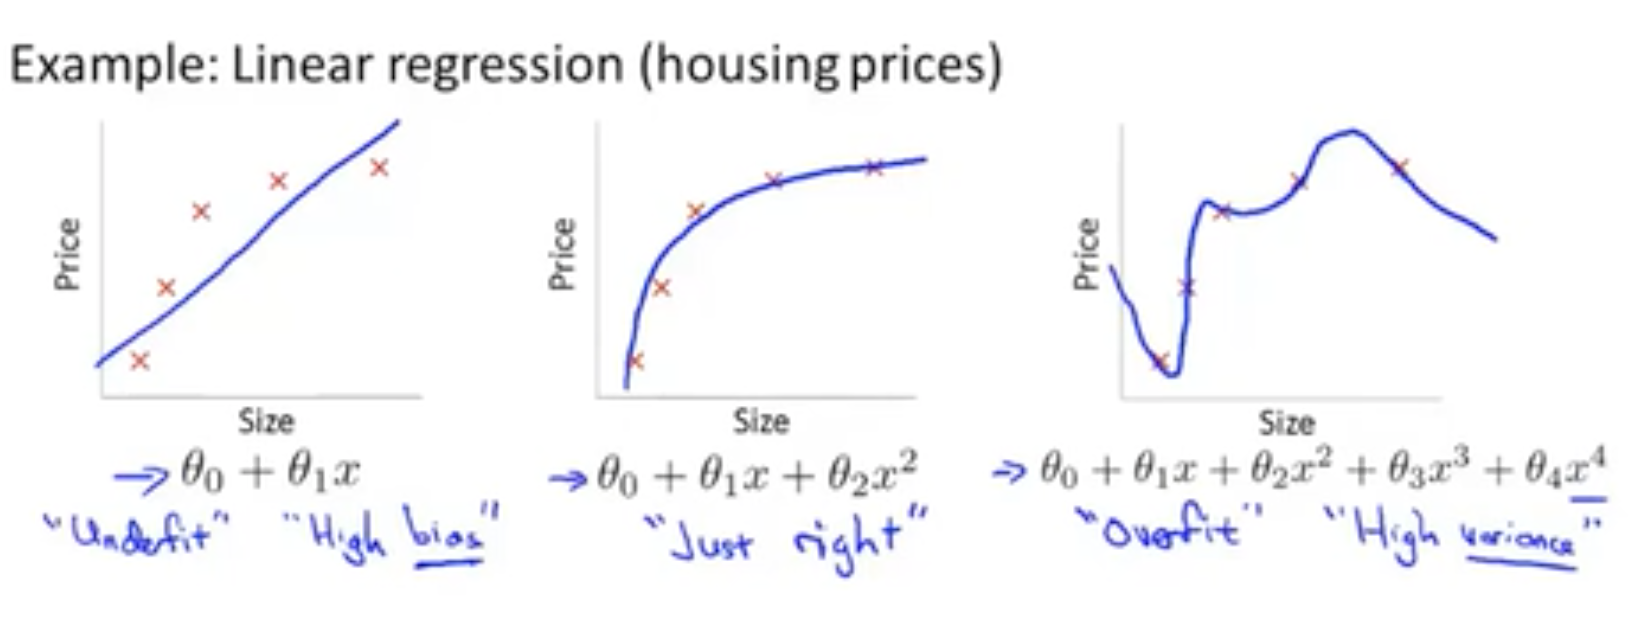
\includegraphics[width=0.8\linewidth]{figs/Chap_5_img1.png}
\end{figure}

同样地，逻辑回归也可能产生过拟合：

\begin{figure}[H]
    \centering
    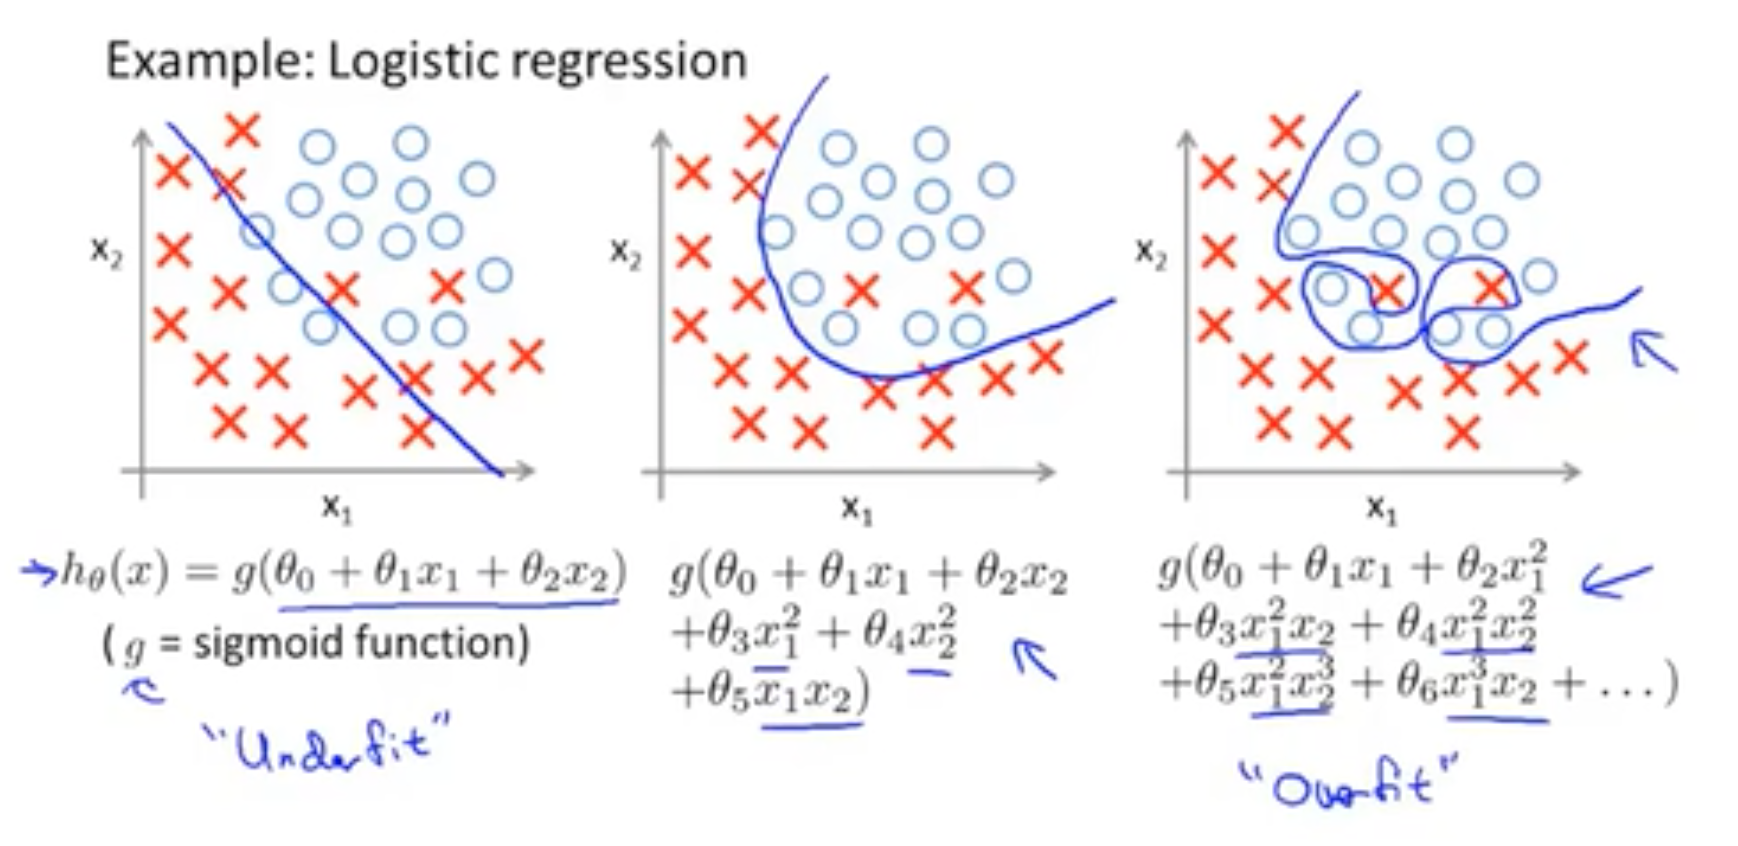
\includegraphics[width=0.8\linewidth]{figs/Chap_5_img2.png}
\end{figure}

解决过拟合的方法有很多，这里学习正则化方法（Regularization）。


\subsection{正则化}

仍然以多项式回归为例，如果我们的假设函数为：$h_\theta(x)=\theta_0+\theta_1x+\theta_2x^2+\theta_3x^3+\theta_4x^4$，而其中的高阶项 $\theta_3,\theta_4$ 导致了过拟合问题，那么我们自然希望 $\theta_3$ 和 $\theta_4$ 越小越好。此时，我们只需要对代价函数做出一点修改：$J(\theta)=\frac{1}{2m}\left[\sum\limits_{i=1}^m\left(h_\theta(x^{(i)})-y^{(i)}\right)^2+1000\theta_3^2+1000\theta_4^2\right]$，这样当 $J(\theta)$ 取最小时，$\theta_3$ 和 $\theta_4$ 都接近于 $0$，我们也就达到了目的。

一般地，我们并不知道究竟应该对哪些参数做出“惩罚”，所以我们设代价函数为：
\[
J(\theta)=\frac{1}{m}\sum_{i=1}^m\text{Cost}\left(h_\theta(x^{(i)})-y^{(i)}\right)+\frac{\lambda}{2m}\sum_{j=1}^n\theta_j^2
\]
其中，$\lambda$ 是正则化参数，$\lambda\sum\limits_{j=1}^n\theta_j^2$ 是正则化项。即我们对\textbf{除了 $\theta_0$ 以外}的参数都做“惩罚”。

如何理解这个代价函数呢？使前一项 $\frac{1}{m}\sum\limits_{i=1}^m\text{Cost}\left(h_\theta(x^{(i)})-y^{(i)}\right)$ 尽可能小是为了去拟合数据集中的数据，使正则化项 $\frac{\lambda}{2m}\sum\limits_{j=1}^n\theta_j^2$ 尽可能小是为了减小各 $\theta_j$ 以避免过拟合，而 $\lambda$ 就是在二者之间权衡的参数。如果 $\lambda$ 很大，意味着正则化项占主要地位，有可能导致所有的 $\theta_j$ 都太小了而无法拟合好数据，即欠拟合；如果 $\lambda$ 很小，意味着拟合数据占主要地位，就有可能过拟合。所以一个合适的正则化参数 $\lambda$ 非常重要。


\paragraph{线性回归的正则化}

线性回归的含有正则化项的代价函数为：
\begin{align*}
J(\theta)&=\frac{1}{2m}\left[\sum_{i=1}^m\left(h_\theta(x^{(i)})-y^{(i)}\right)^2+\lambda\sum_{j=1}^n\theta_j^2\right]\\
&=\frac{1}{2m}\left[\sum_{i=1}^m\left(\theta^Tx^{(i)}-y^{(i)}\right)^2+\lambda\sum_{j=1}^n\theta_j^2\right]
\end{align*}
对其求导：
\[
\frac{\partial J}{\partial \theta_j}=\frac{1}{m}\sum_{i=1}^m\left(\theta^Tx^{(i)}-y^{(i)}\right)x^{(i)}_j+[j\neq 0]\frac{\lambda}{m}\theta_j,\quad j=0,1,\cdots,n
\]
所以梯度下降时，我们的迭代过程为：
\begin{align*}
\theta_j&:=\theta_j-\alpha \frac{\partial J}{\partial \theta_j}\\
&=\theta_j-\alpha \left[\frac{1}{m}\sum_{i=1}^m\left(\theta^Tx^{(i)}-y^{(i)}\right)x^{(i)}_j+\frac{\lambda}{m}\theta_j\right]\\
&=\theta_j\left(1-\alpha\frac{\lambda}{m}\right)-\alpha\frac{1}{m}\sum_{i=1}^m\left(\theta^Tx^{(i)}-y^{(i)}\right)x^{(i)}_j,\quad j=1,\cdots,n
\end{align*}

若不用梯度下降，而是直接用正规方程，即在数学上解它，那么：

为了记号的方便，我们先假定对 $\theta_0$ 也进行“惩罚”。首先将 $J(\theta)$ 写作矩阵形式：
\begin{align*}
J(\theta)&=\frac{1}{2m}\left[\sum_{i=1}^m\left(\theta^Tx^{(i)}\right)^2-2\sum_{i=1}^m\theta^Tx^{(i)}y^{(i)}+\sum_{i=1}^m\left(y^{(i)}\right)^2+\lambda\theta^T\theta\right]\\
&=\frac{1}{2m}\left[\left(\theta^TX^T\right)\left(\theta^TX^T\right)^T-2\theta^TX^Ty+y^Ty+\lambda\theta^T\theta\right]\\
&=\frac{1}{2m}\left[\theta^TX^TX\theta-2\theta^TX^Ty+y^Ty+\lambda\theta^T\theta\right]
\end{align*}
然后令
\[
\frac{\partial J}{\partial \theta}=\frac{1}{m}\left[X^TX\theta-X^Ty+\lambda\theta\right]=0
\]
则：
\[
(X^TX+\lambda)\theta=X^Ty
\]
解得：
\[
\theta=(X^TX+\lambda)^{-1}X^Ty
\]
现在把 $j=0$ 的特殊情况考虑进去，那么最后的结果就是：
\[
\theta=\left(X^TX+\lambda\begin{bmatrix}0&&&\\&1&&\\&&\ddots&\\&&&1\end{bmatrix}\right)^{-1}X^Ty
\]


\paragraph{逻辑回归的正则化}

逻辑回归的含有正则化项的代价函数为：
\begin{align*}
J(\theta)&=-\frac{1}{m}\sum_{i=1}^m\left[y^{(i)}\ln(h_\theta(x^{(i)}))+(1-y^{(i)})\ln(1-h_\theta(x^{(i)}))\right]+\frac{\lambda}{2m}\sum_{j=1}^n\theta_j^2\\
&=\frac{1}{m}\sum_{i=1}^m\left[y^{(i)}\ln\left(1+e^{-\theta^Tx^{(i)}}\right)+\left(1-y^{(i)}\right)\ln\left(1+e^{\theta^Tx^{(i)}}\right)\right]+\frac{\lambda}{2m}\sum_{j=1}^n\theta_j^2
\end{align*}
对其求导：
\[
\frac{\partial J}{\partial \theta_j}=\frac{1}{m}\sum_{i=1}^m\left(h_\theta(x^{(i)})-y^{(i)}\right)x^{(i)}_j+[j\neq 0]\frac{\lambda}{m}\theta_j,\quad j=0,1,\cdots,n
\]
所以梯度下降时，我们的迭代过程为：
\begin{align*}
\theta_0&:=\theta_0-\alpha\frac{\partial J}{\partial\theta_j}\\
&=\theta_0-\alpha\frac{1}{m}\sum_{i=1}^m\left(h_\theta(x^{(i)})-y^{(i)}\right)x_0^{(i)}
\\
\theta_j&:=\theta_j-\alpha \frac{\partial J}{\partial \theta_j}\\
&=\theta_j-\alpha \left[\frac{1}{m}\sum_{i=1}^m\left(h_\theta(x^{(i)})-y^{(i)}\right)x^{(i)}_j+\frac{\lambda}{m}\theta_j\right]\\
&=\theta_j\left(1-\alpha\frac{\lambda}{m}\right)-\alpha\frac{1}{m}\sum_{i=1}^m\left(h_\theta(x^{(i)})-y^{(i)}\right)x^{(i)}_j,\quad j=1,\cdots,n
\end{align*}

和线性回归一样，我们更希望将上面的式子写作矩阵形式。

注意：以下表达式与 \texttt{numpy} 的矩阵形式相对应，即存在 "broadcast" 的表示方式，在数学上不一定严谨。



\paragraph{代价函数的矩阵形式}

回顾逻辑回归的代价函数：
\[
J(\theta)=\frac{1}{m}\sum_{i=1}^m\left[-y^{(i)}\ln(h_\theta(x^{(i)}))-(1-y^{(i)})\ln(1-h_\theta(x^{(i)}))\right]
\]
其中，
\[
h_\theta(x)=g(\theta^Tx)=\frac{1}{1+e^{-\theta^Tx}}
\]
设：
\[
X=\begin{bmatrix}(x^{(1)})^T\\(x^{(2)})^T\\\vdots\\(x^{(m)})^T\end{bmatrix}\quad \theta=\begin{bmatrix}\theta_0\\\theta_1\\\vdots\\\theta_n\end{bmatrix}\quad y=\begin{bmatrix}y^{(0)}\\y^{(1)}\\\vdots\\y^{(m)}\end{bmatrix}
\]
于是：
\[
X\theta=\begin{bmatrix}(x^{(1)})^T\theta\\(x^{(2)})^T\theta\\\vdots\\(x^{(m)})^T\theta\end{bmatrix}=\begin{bmatrix}\theta^T(x^{(1)})\\\theta^T(x^{(2)})\\\vdots\\\theta^T(x^{(m)})\end{bmatrix}
\]
所以，设：
\[
h'_\theta(X)=1/(1+e^{-X\theta})\in\mathbb R^{m}
\]
于是：
\[
J(\theta)=-\frac{1}{m}\left[y^T\ln(h'_\theta(X))+(1-y^T)\ln(1-h'_\theta(X))\right]
\]


\paragraph{代价函数偏导的矩阵形式}

逻辑回归的代价函数的偏导函数向量：
\[
\frac{\partial J}{\partial \theta}=\frac{1}{m}\sum_{i=1}^m\left[\left(h_\theta(x^{(i)})-y^{(i)}\right)x^{(i)}\right]=\frac{1}{m}X^T(h'_\theta(X)-y)
\]


\paragraph{正则化后的矩阵形式}

回顾正则化后的逻辑回归代价函数及其偏导：
\begin{align*}
J(\theta)&=\frac{1}{m}\sum_{i=1}^m\left[-y^{(i)}\ln(h_\theta(x^{(i)}))-(1-y^{(i)})\ln(1-h_\theta(x^{(i)}))\right]+\frac{\lambda}{2m}\sum_{j=1}^n\theta_j^2\\
\frac{\partial J}{\partial \theta}&=\frac{1}{m}\sum_{i=1}^m\left(h_\theta(x^{(i)})-y^{(i)}\right)x^{(i)}+\frac{\lambda}{m}\hat\theta
\end{align*}
注意，这里 $\hat\theta=\begin{bmatrix}0\\\theta_1\\\vdots\\\theta_n\end{bmatrix}$，即在 $\theta$ 中将 $\theta_0$ 换成 $0$. 

有了之前的推导，就容易写出正则化后的矩阵形式了：
\begin{align*}
J(\theta)&=-\frac{1}{m}\left[y^T\ln(h'_\theta(X))+(1-y^T)\ln(1-h'_\theta(X))\right]+\frac{\lambda}{2m}\hat\theta^T\hat\theta\\
\frac{\partial J}{\partial \theta}&=\frac{1}{m}X^T(h'_\theta(X)-y)+\frac{\lambda}{m}\hat\theta
\end{align*}
这也是我们使用 `numpy` 实现正则化逻辑回归时的表达式。


\subsection{代码实现}

首先还是来看一下数据集：

\begin{figure}[H]
    \centering
    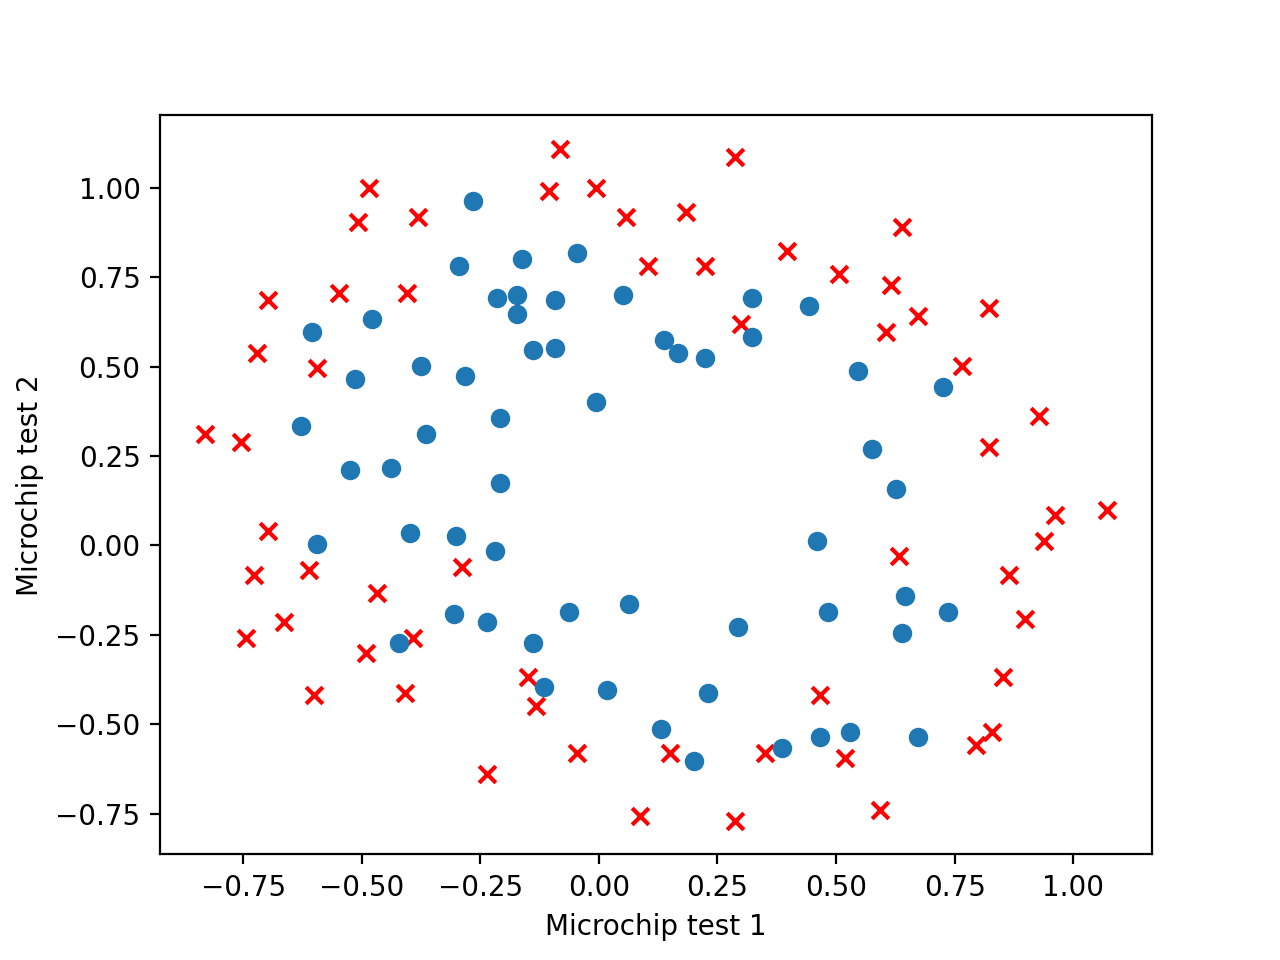
\includegraphics[width=0.5\linewidth]{figs/Chap_5_Figure_0.png}
\end{figure}

显然，我们需要用一个多项式去进行逻辑回归，这里将数据的两维都扩充为 $3$ 次，形成有 $16$ 维特征的数据，然后进行逻辑回归。

\begin{lstlisting}[language=Python]
import numpy as np
import matplotlib.pyplot as plt

alpha = 0.01
lamb = 1
iteration = 1000000
Z = []

def h(Theta, x):
	return 1 / (1 + np.exp(-np.matmul(Theta.T, x)[0][0]))

def h_(Theta, X):
	return 1 / (1 + np.exp(-np.matmul(X, Theta)))

def J_reg(Theta, X, y):
	tmp = h_(Theta, X)
	return (-(np.matmul(y.T, np.log(tmp)) + np.matmul(1 - y.T, np.log(1 - tmp))) / m\
		 + lamb / 2 / m * np.matmul(Theta.T, Theta))[0][0]

def partJ_reg(Theta, X, y):
	return (np.matmul(X.T, h_(Theta, X) - y) + lamb * np.vstack((np.zeros((1, 1)), Theta[1:, :]))) / m

def GradientDescent(X, Y):
	T = np.zeros((n, 1))
	for t in range(iteration):
		T = T - alpha * partJ_reg(T, X, Y)
		Z.append(J_reg(T, X, Y))
	return T

def extend(x1, x2):
	X = []
	for j in range(4):
		for k in range(4):
			X.append(np.power(x1, j) * np.power(x2, k))
	return X

data = np.genfromtxt("ex2data2.txt", delimiter = ',')
(m, n) = data.shape
Y = data[:, -1:]
n = 16
X = np.zeros((m, n))
for i in range(m):
	X[i] = extend(data[i][0], data[i][1])

T = GradientDescent(X, Y)
print(T.T)
print(J_reg(T, X, Y))

#============================== draw the picture ==============================#

def calc(x1, x2):
	res = np.zeros((x1.shape[0], x1.shape[1]))
	for ix in range(x1.shape[0]):
		for iy in range(x1.shape[1]):
			tmp = np.array(extend(x1[ix][iy], x2[ix][iy]), ndmin = 2)
			res[ix][iy] = h(T, tmp.T)
	return res

minx1, maxx1 = data[:, 0].min(), data[:, 0].max()+0.1
minx2, maxx2 = data[:, 1].min(), data[:, 1].max()+0.1
delta = 0.01
x1, x2 = np.meshgrid(np.arange(minx1, maxx1, delta), np.arange(minx2, maxx2, delta))

p1 = plt.subplot(121)
plt.contour(x1, x2, calc(x1, x2), [0.5], colors = 'magenta')

X0 = data[data[:, -1] == 0, :]
X1 = data[data[:, -1] == 1, :]
p1.set_title("lambda = " + str(lamb))
p1.set_xlabel("Microchip test 1")
p1.set_ylabel("Microchip test 2")
p1.scatter(X0[:, 0:1], X0[:, 1:2], marker = 'x', c = 'r')
p1.scatter(X1[:, 0:1], X1[:, 1:2], marker = 'o')

p2 = plt.subplot(122)
p2.plot(range(1, iteration+1), Z)
p2.set_title("lambda = " + str(lamb))
p2.set_xlabel("Iteration")
p2.set_ylabel("Cost")

plt.show()
\end{lstlisting}

以下是 $\lambda=0,1,5$ 的回归结果和收敛情况：

\begin{figure}[H]
    \centering
    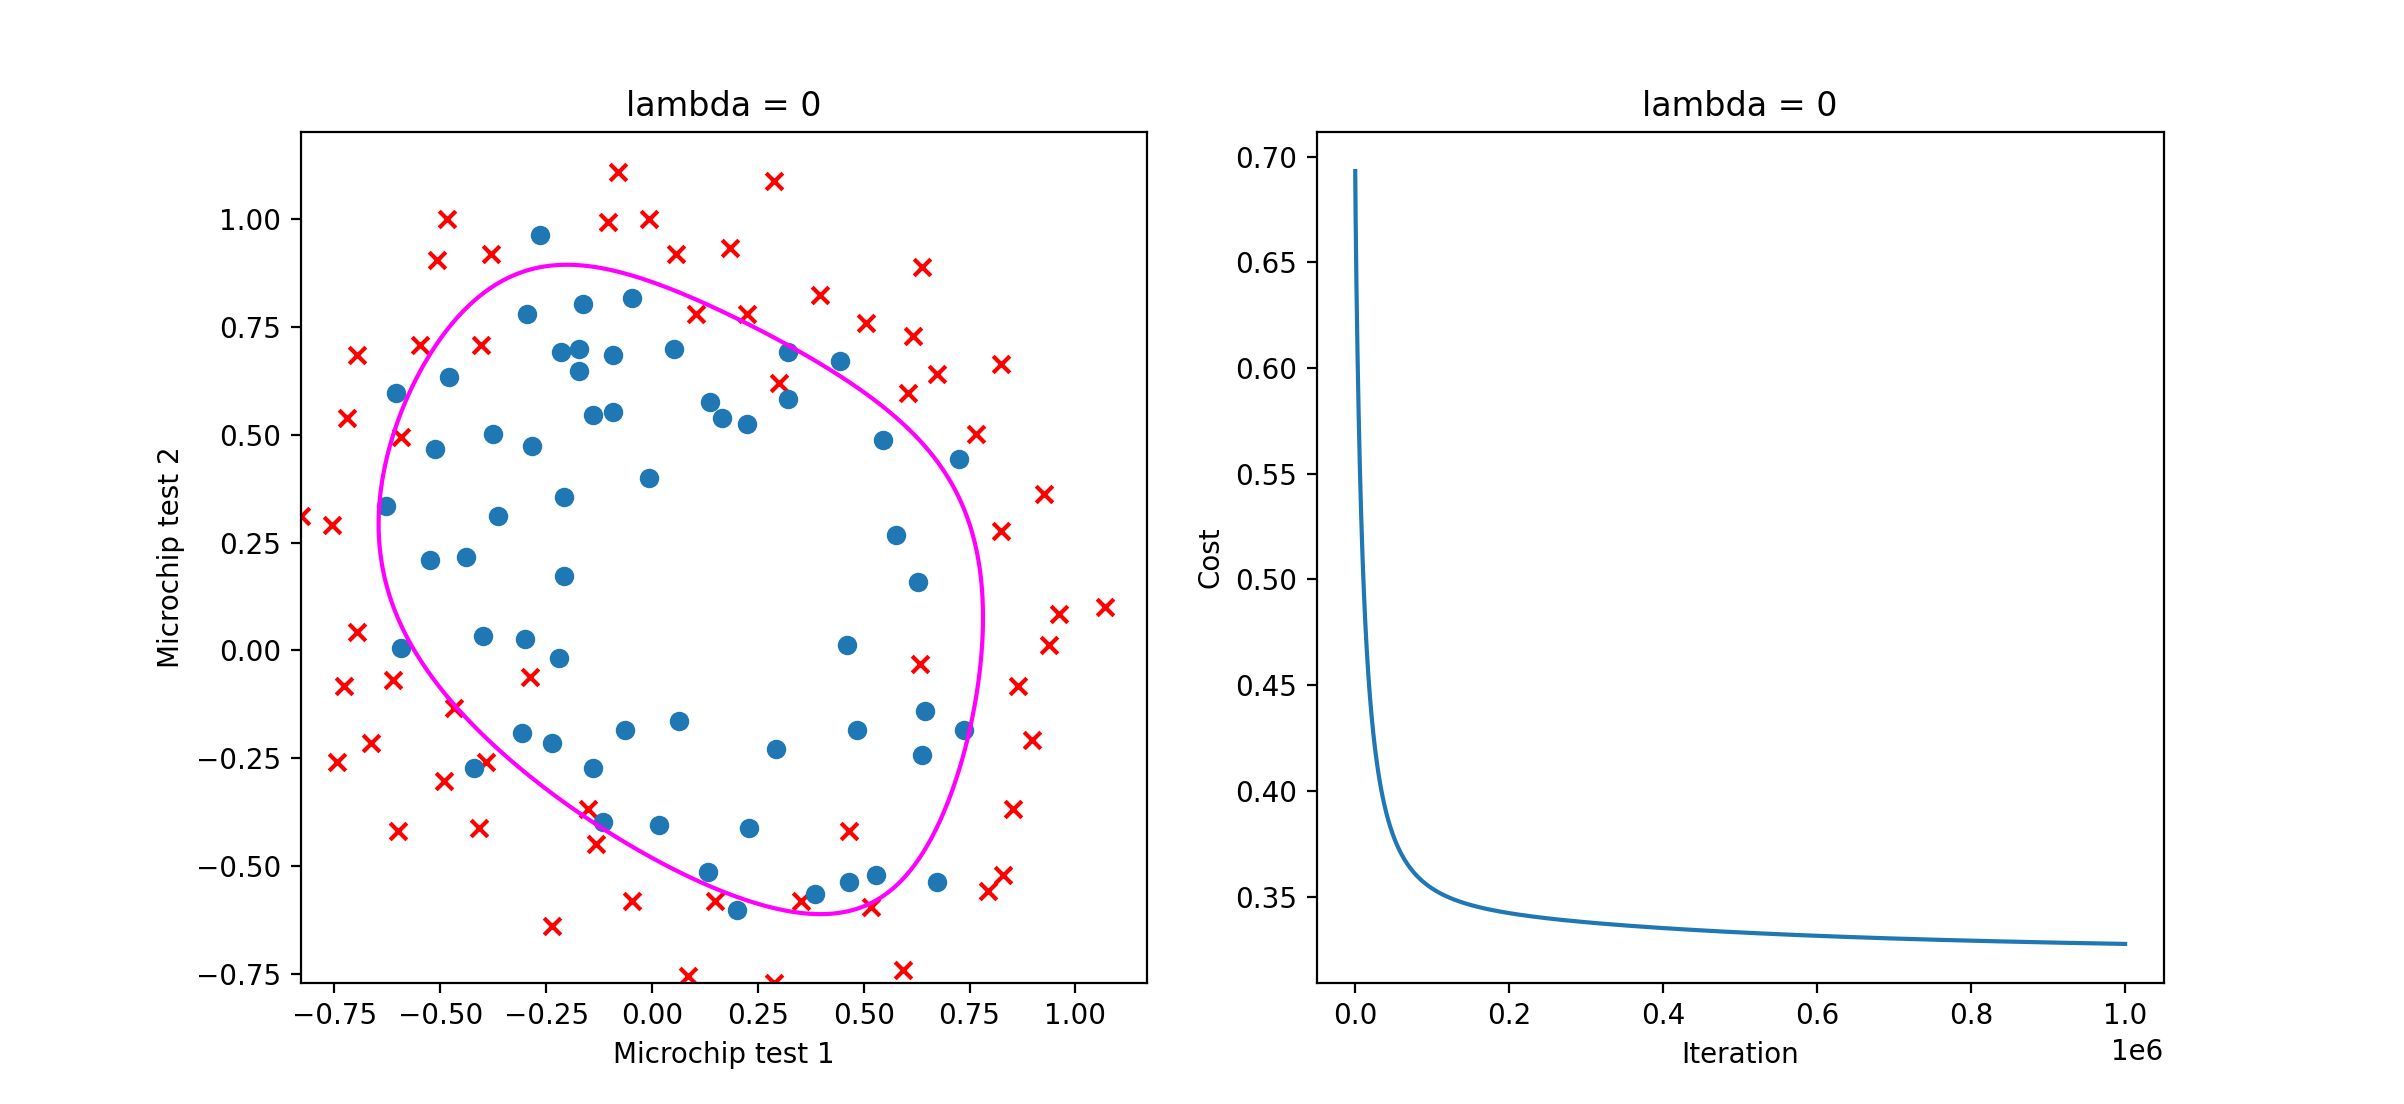
\includegraphics[width=\linewidth]{figs/Chap_5_Figure_11.png}
\end{figure}

\begin{figure}[H]
    \centering
    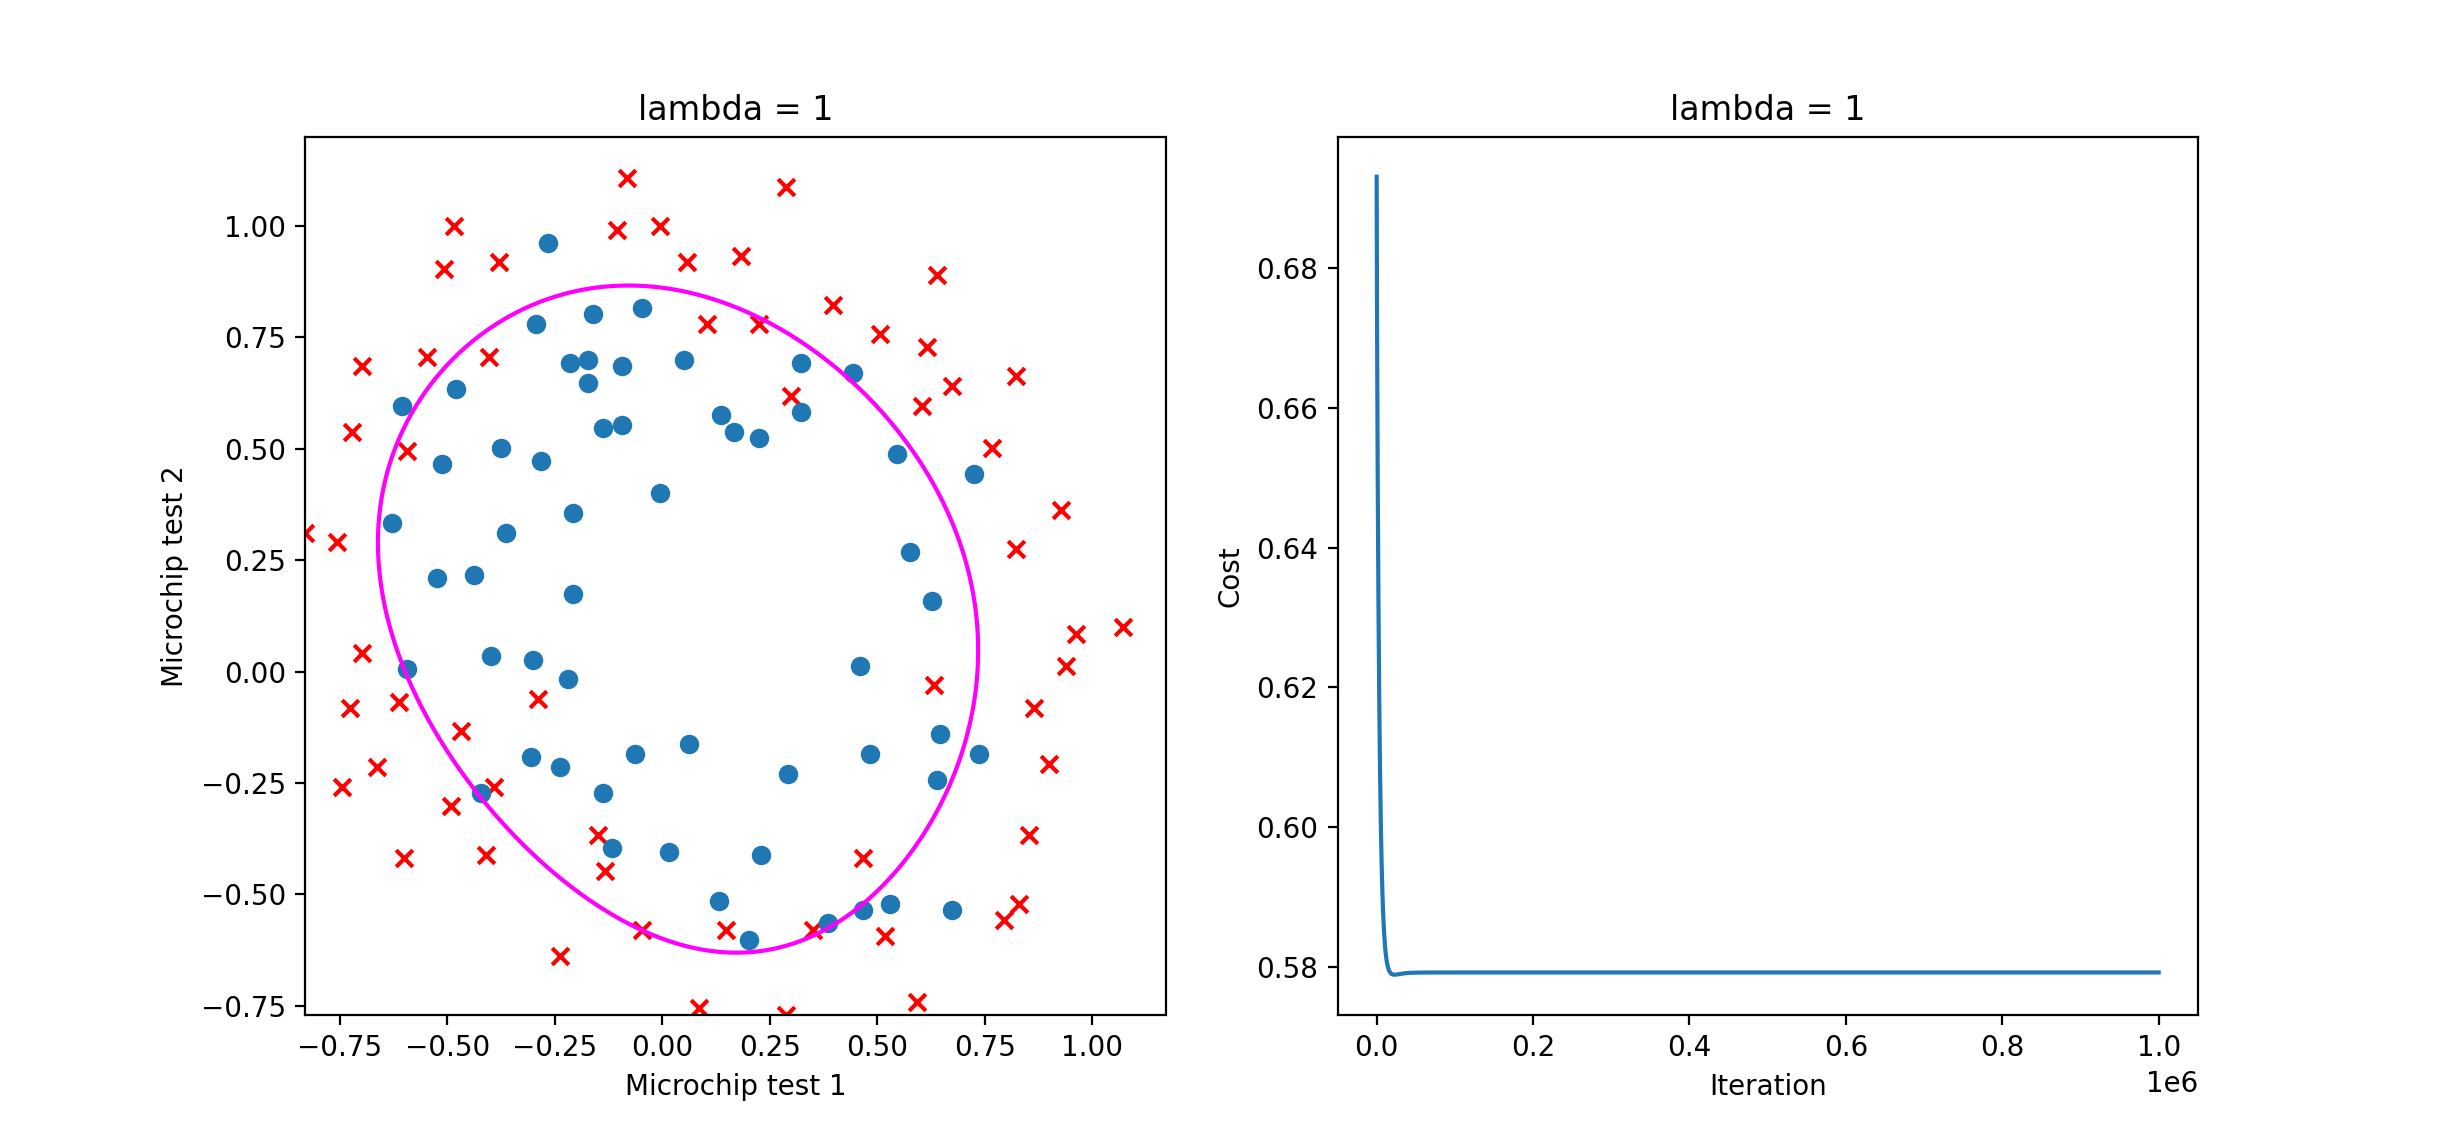
\includegraphics[width=\linewidth]{figs/Chap_5_Figure_12.png}
\end{figure}

\begin{figure}[H]
    \centering
    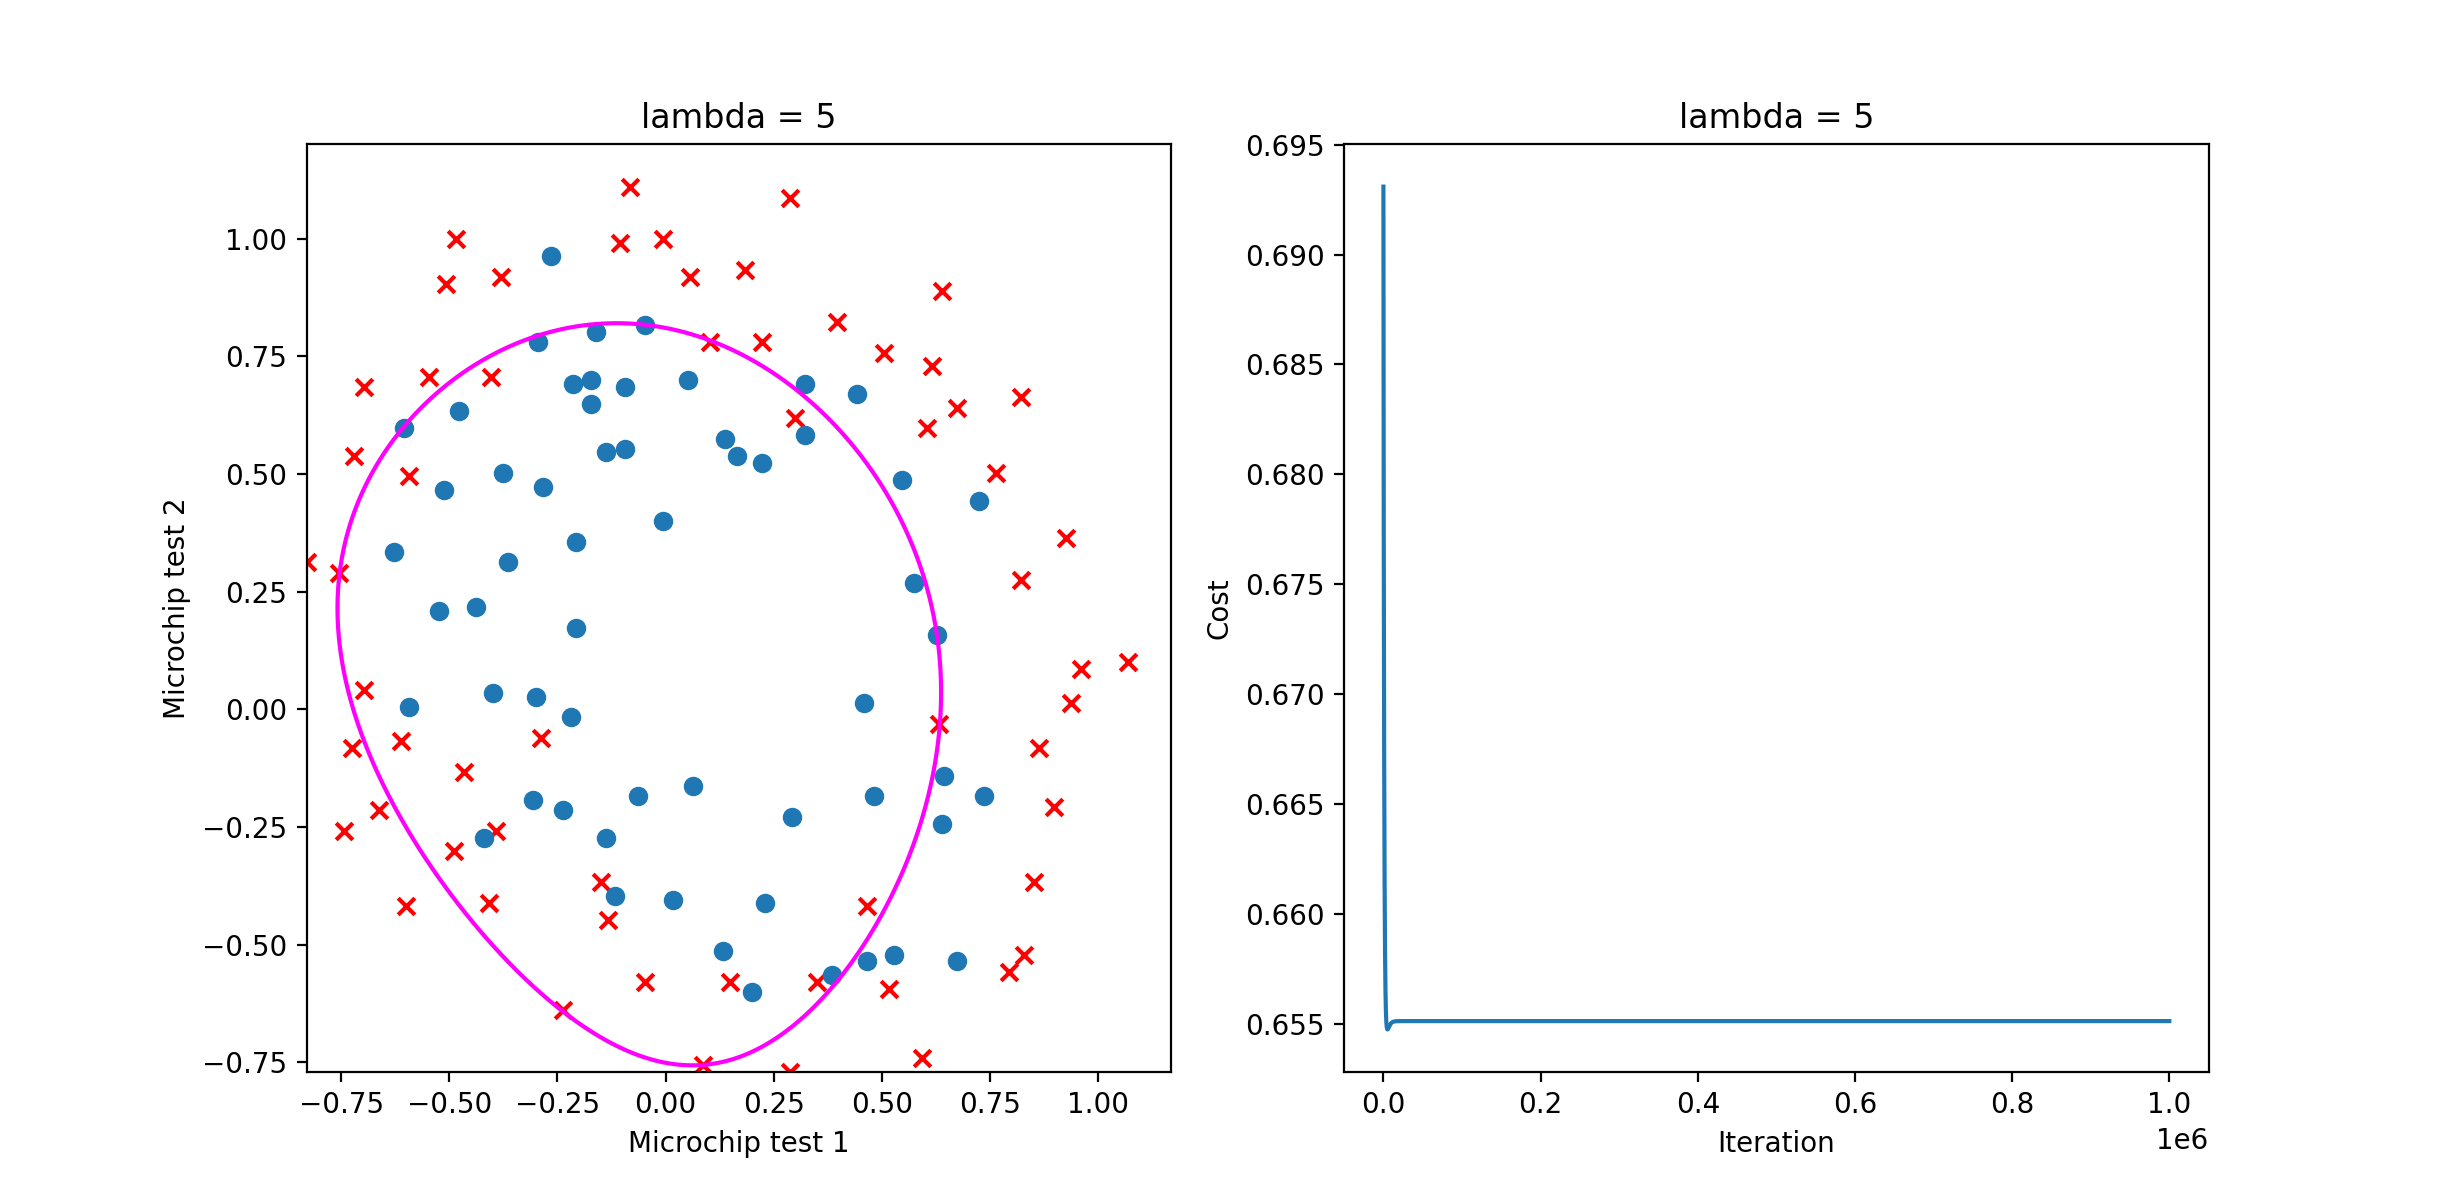
\includegraphics[width=\linewidth]{figs/Chap_5_Figure_13.png}
\end{figure}


接下来我换了一个生成特征的方式：

\begin{lstlisting}[language=Python]
def extend(x1, x2):
	X = []
	for j in range(6 + 1):
		for k in range(j + 1):
			X.append(np.power(x1, k) * np.power(x2, j-k))
	return X
\end{lstlisting}

结果如下：

\begin{figure}[H]
    \centering
    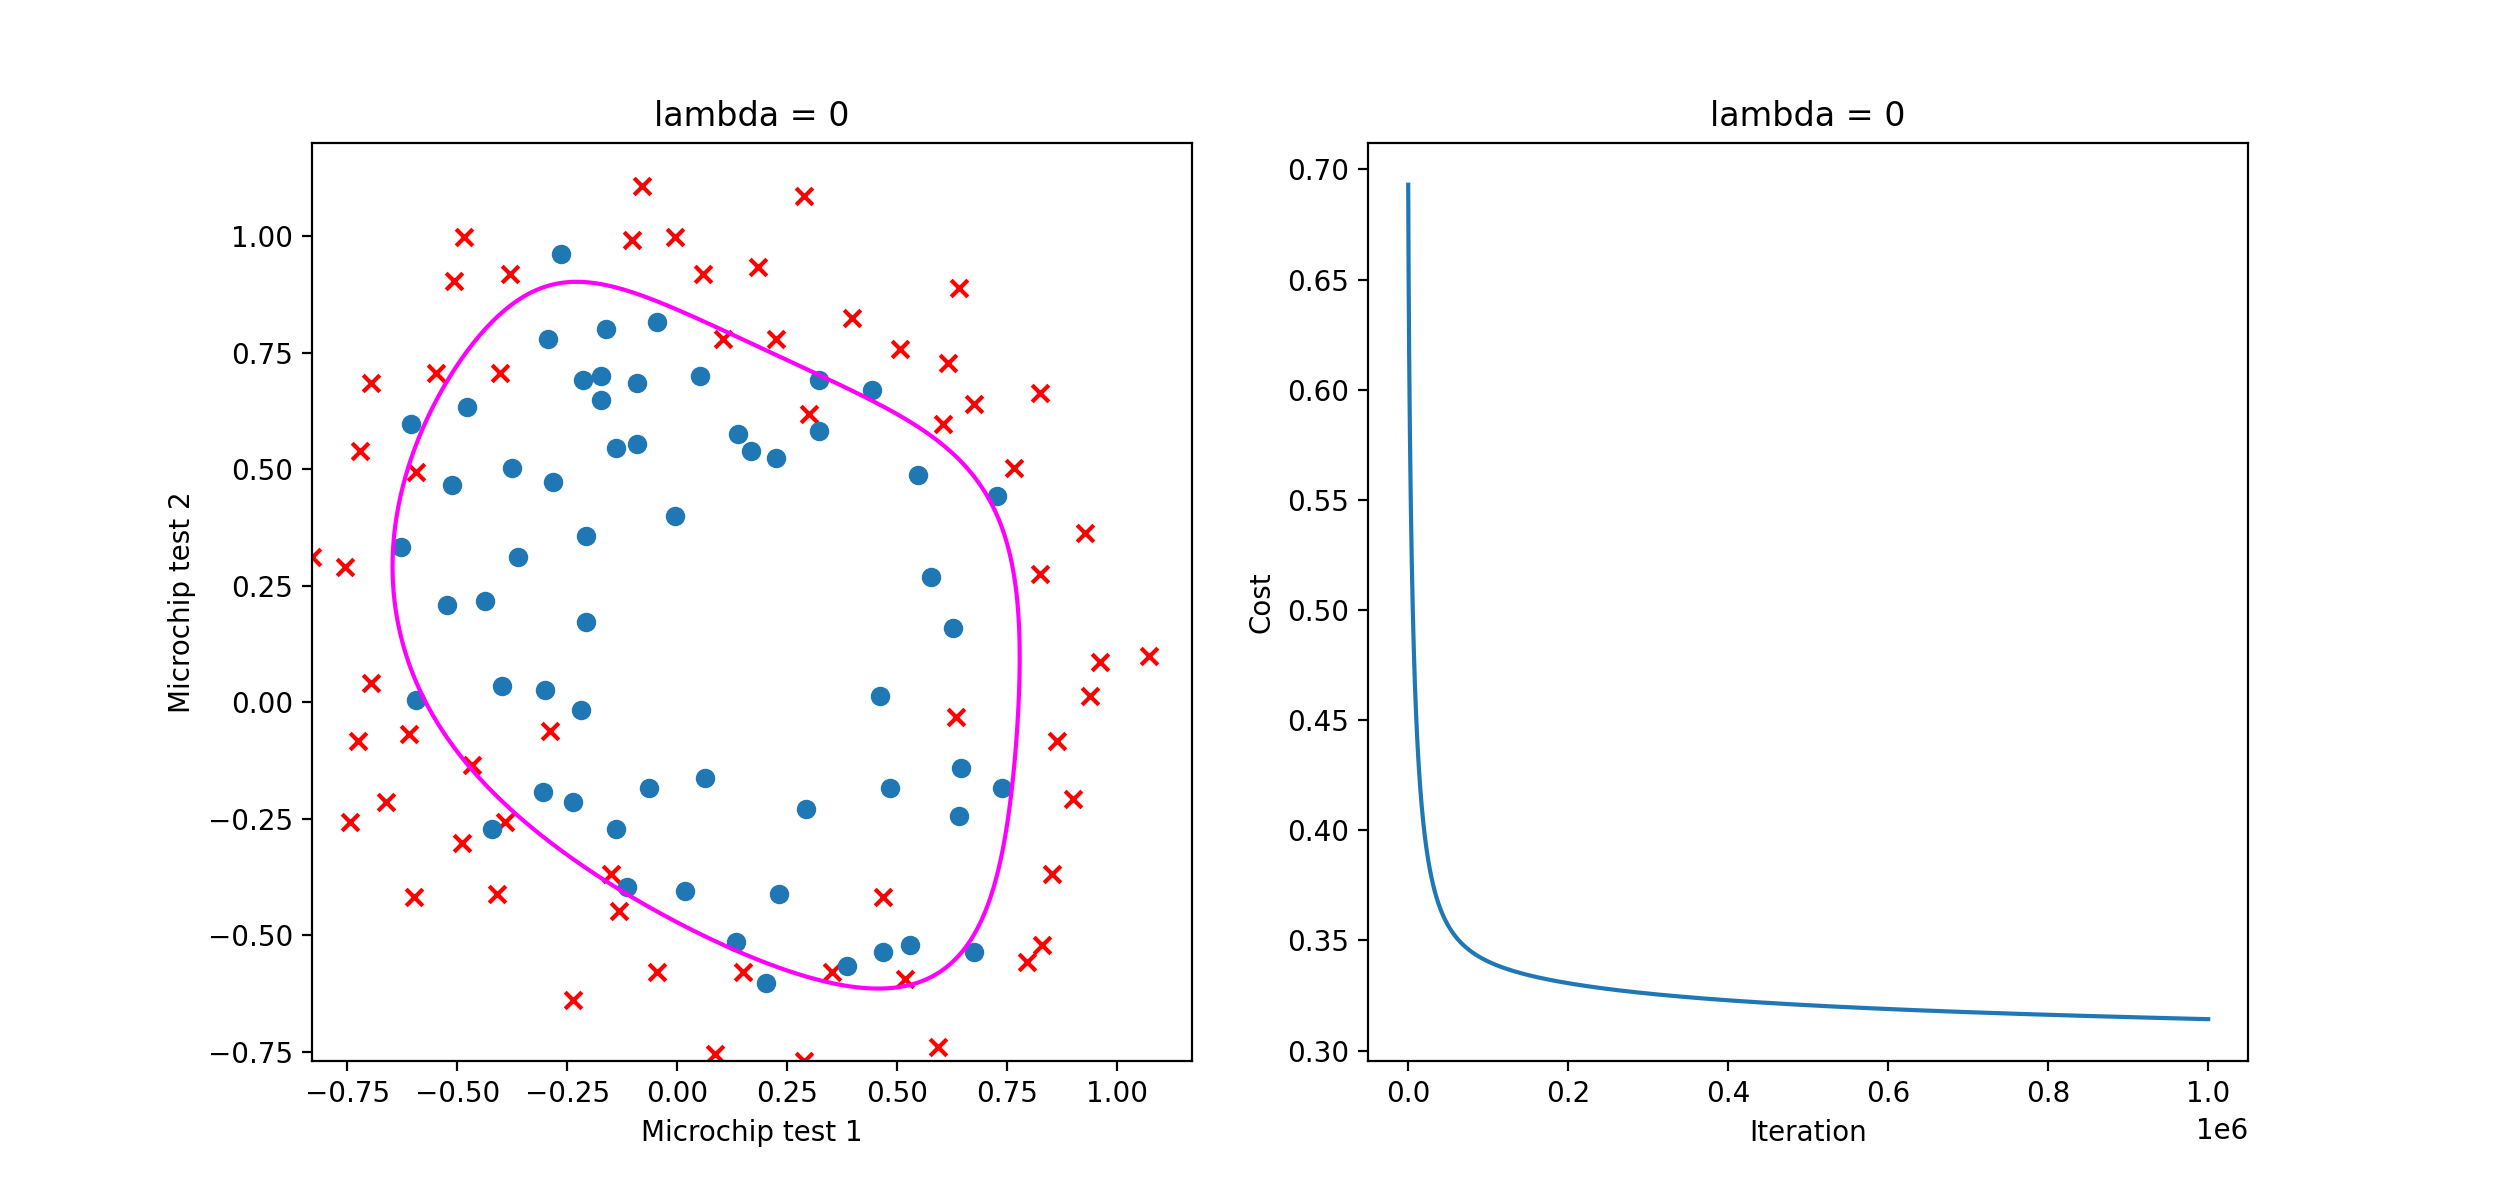
\includegraphics[width=\linewidth]{figs/Chap_5_Figure_21.png}
\end{figure}

\begin{figure}[H]
    \centering
    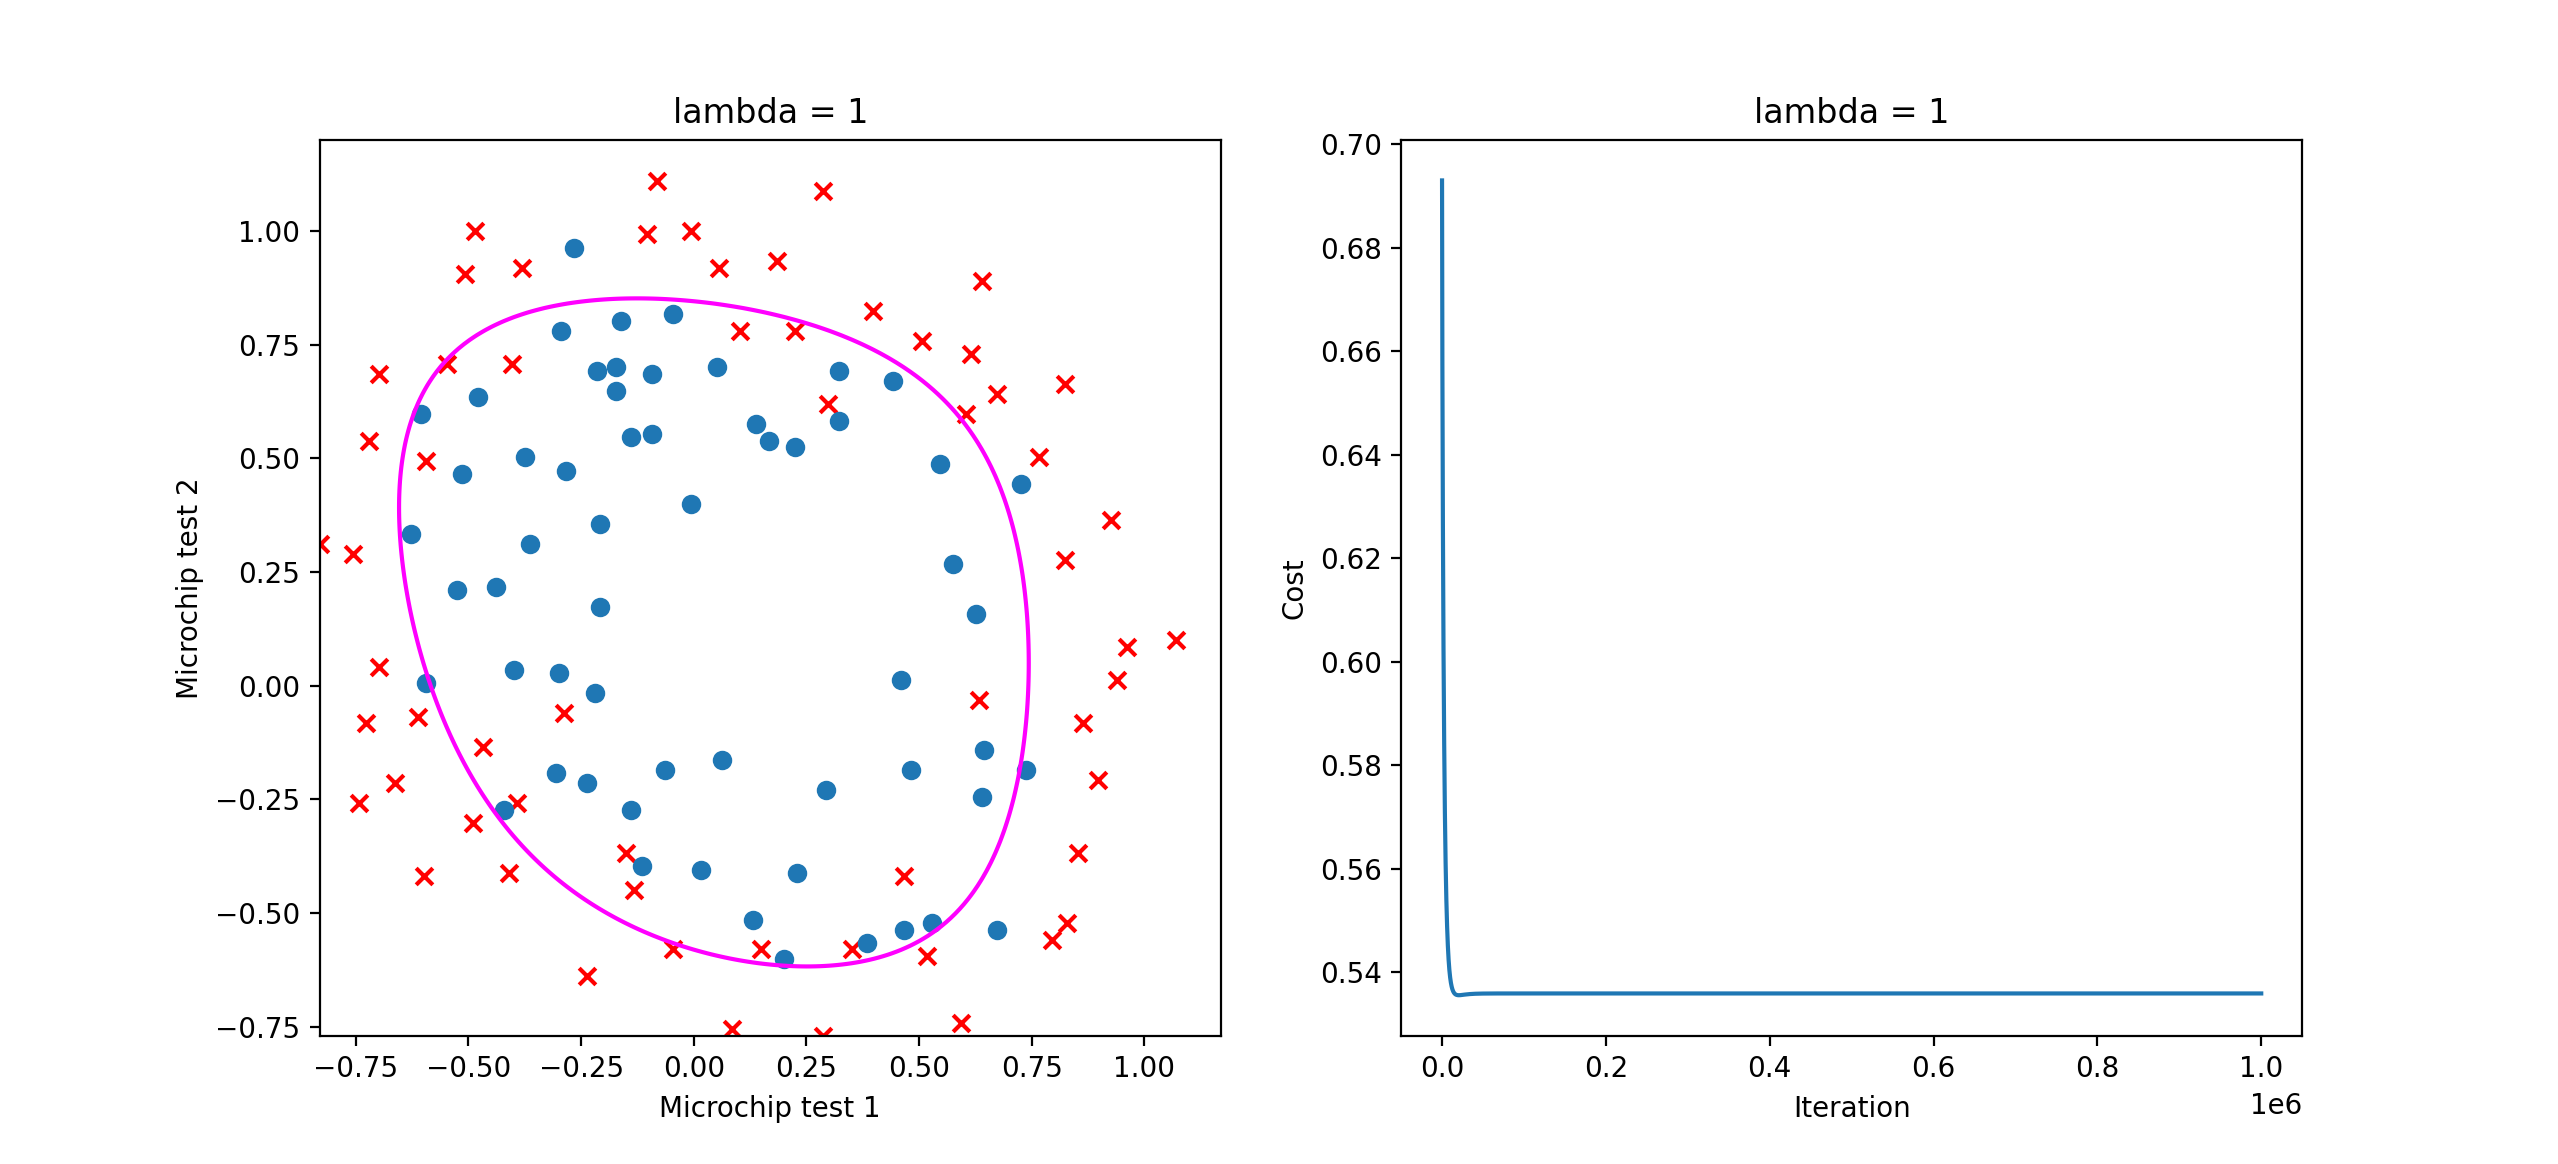
\includegraphics[width=\linewidth]{figs/Chap_5_Figure_22.png}
\end{figure}

\begin{figure}[H]
    \centering
    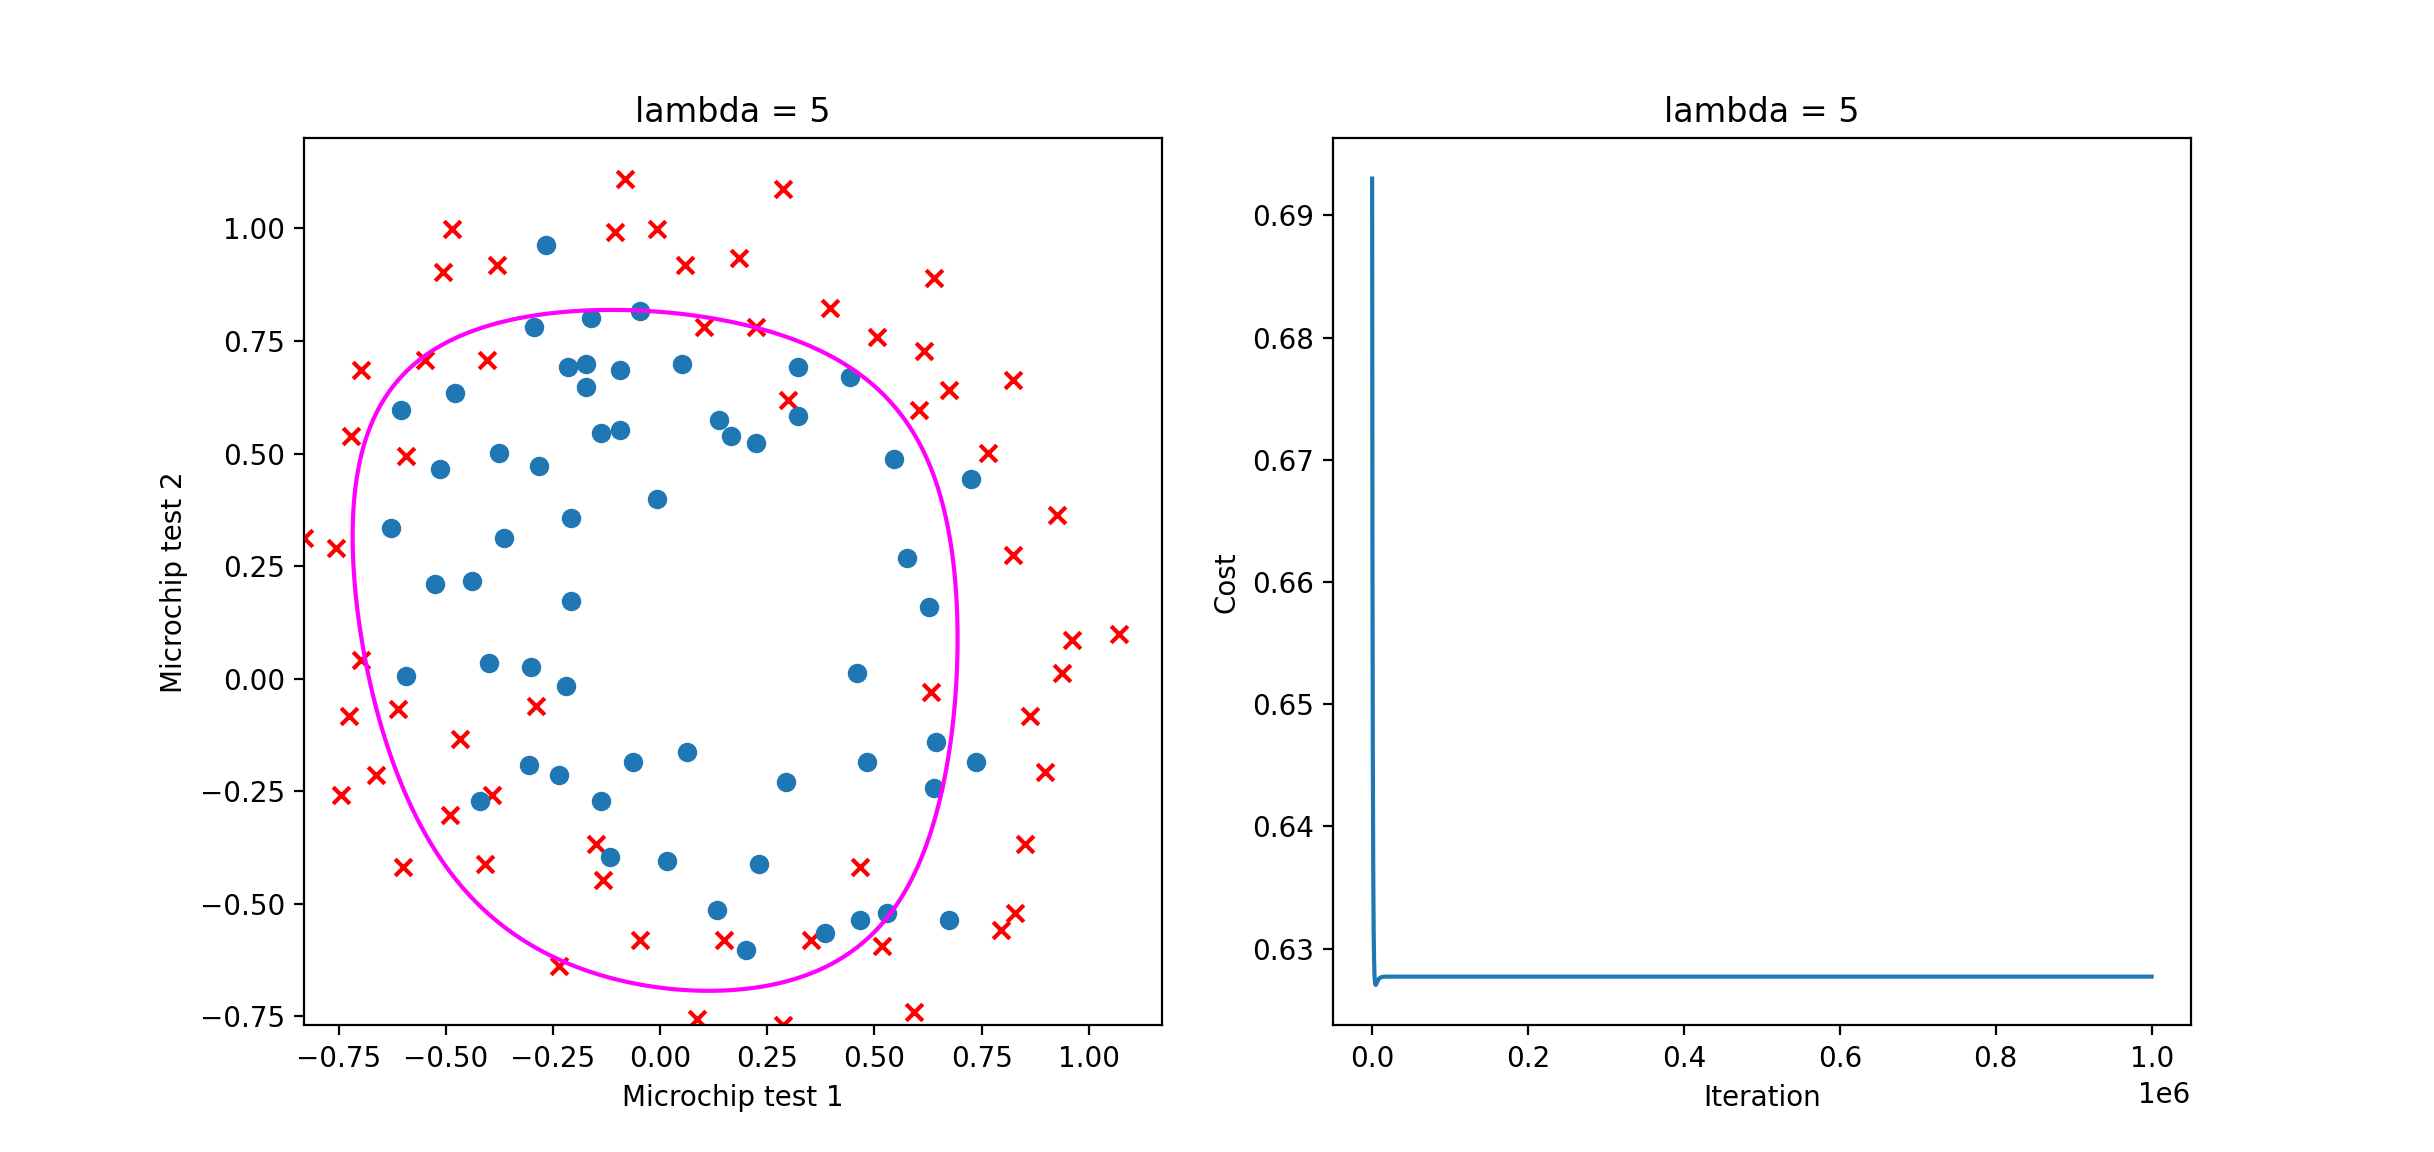
\includegraphics[width=\linewidth]{figs/Chap_5_Figure_23.png}
\end{figure}
